% !TEX program = xelatex
% ============================================================
%  毕业答辩 Beamer（15 分钟，~16 张幻灯片）
%  编译：xelatex slides.tex（跑两次）
% ============================================================
\documentclass[aspectratio=169,10pt,fontset=none]{ctexbeamer}

% ---------- 主题 ----------
\usetheme{Madrid}
\usecolortheme{whale}
\setbeamertemplate{navigation symbols}{}
\setbeamertemplate{caption}[numbered]
\setbeamerfont{frametitle}{size=\large}
\setbeamerfont{title}{size=\LARGE}

% ---------- 共享 preamble ----------
% !TEX program = xelatex
% ---------- 共享 preamble ----------
% slides 与 script 共用。仅拉 _figpreamble.tex 的颜色宏 + tikz + pgfplots + subcaption。
% 不 \input 毕业论文/preamble.tex（避免 ctexbook 与 ctexbeamer/ctexart 冲突）。

% ---------- 字体 ----------
\def\ProjectFontDir{../fonts}
% Project-local font setup for XeLaTeX.
% Callers may set \ProjectFontDir before \input'ing this file.
\providecommand{\ProjectFontDir}{../fonts}

\setmainfont[
  Path = \ProjectFontDir/tex-gyre/,
  Extension = .otf,
  UprightFont = *-regular,
  BoldFont = *-bold,
  ItalicFont = *-italic,
  BoldItalicFont = *-bolditalic,
  Ligatures = TeX
]{texgyretermes}

\setCJKmainfont[
  Path = \ProjectFontDir/fandol/,
  Extension = .otf,
  BoldFont = FandolSong-Bold,
  ItalicFont = FandolKai-Regular
]{FandolSong-Regular}
\setCJKsansfont[
  Path = \ProjectFontDir/fandol/,
  Extension = .otf,
  BoldFont = FandolHei-Bold,
  ItalicFont = FandolKai-Regular
]{FandolHei-Regular}
\setCJKmonofont[
  Path = \ProjectFontDir/fandol/,
  Extension = .otf,
  ItalicFont = FandolKai-Regular
]{FandolFang-Regular}

\setCJKfamilyfont{zhsong}[
  Path = \ProjectFontDir/fandol/,
  Extension = .otf,
  BoldFont = FandolSong-Bold
]{FandolSong-Regular}
\setCJKfamilyfont{zhsongb}[
  Path = \ProjectFontDir/fandol/,
  Extension = .otf
]{FandolSong-Bold}
\setCJKfamilyfont{zhhei}[
  Path = \ProjectFontDir/fandol/,
  Extension = .otf,
  BoldFont = FandolHei-Bold,
  ItalicFont = FandolKai-Regular
]{FandolHei-Regular}
\setCJKfamilyfont{zhheib}[
  Path = \ProjectFontDir/fandol/,
  Extension = .otf
]{FandolHei-Bold}
\setCJKfamilyfont{zhfs}[
  Path = \ProjectFontDir/fandol/,
  Extension = .otf
]{FandolFang-Regular}
\setCJKfamilyfont{zhkai}[
  Path = \ProjectFontDir/fandol/,
  Extension = .otf
]{FandolKai-Regular}

\ExplSyntaxOn
\cs_if_exist:NT \ctex_punct_set:n
  {
    \ctex_punct_set:n { fandol }
    \ctex_punct_map_family:nn   { \CJKrmdefault         } { zhsong  }
    \ctex_punct_map_family:nn   { \CJKsfdefault         } { zhhei   }
    \ctex_punct_map_family:nn   { \CJKttdefault         } { zhfs    }
    \ctex_punct_map_bfseries:nn { \CJKrmdefault, zhsong } { zhsongb }
    \ctex_punct_map_bfseries:nn { \CJKsfdefault, zhhei  } { zhheib  }
    \ctex_punct_map_itshape:nn  { \CJKrmdefault         } { zhkai   }
  }
\ExplSyntaxOff

\providecommand{\songti}{}
\providecommand{\heiti}{}
\providecommand{\fangsong}{}
\providecommand{\kaishu}{}
\renewcommand{\songti}{\CJKfamily{zhsong}}
\renewcommand{\heiti}{\CJKfamily{zhhei}}
\renewcommand{\fangsong}{\CJKfamily{zhfs}}
\renewcommand{\kaishu}{\CJKfamily{zhkai}}


% ---------- 宏包 ----------
\usepackage{amsmath,amssymb}
\usepackage{booktabs}
\usepackage{array}
\usepackage{multirow}
\usepackage{tikz}
\usetikzlibrary{shapes.geometric, arrows.meta, positioning, fit, backgrounds, calc, patterns, decorations.pathreplacing}
\usetikzlibrary{external}
\tikzexternalize
\usepackage{pgfplots}
\pgfplotsset{compat=1.18}
\usepgfplotslibrary{fillbetween}
\pgfplotsset{table/search path={../图片/, ../图片/data/, ../}}
\usepackage{xcolor}
\usepackage{colortbl}
\usepackage{caption}
\usepackage{subcaption}
\usepackage{adjustbox}
\usepackage[absolute,overlay]{textpos}
\usepackage[skins]{tcolorbox}

% ---------- 统一调色板（与 图片/_figpreamble.tex 同步） ----------
\definecolor{deepblue}{RGB}{81, 132, 178}
\definecolor{lightblue}{RGB}{170, 212, 248}
\definecolor{skyblue}{RGB}{154, 220, 255}
\definecolor{inputyellow}{RGB}{255, 248, 154}
\definecolor{outputpink}{RGB}{255, 178, 166}
\definecolor{improvedpink}{RGB}{255, 138, 174}
\definecolor{lightpink}{RGB}{241, 167, 181}
\definecolor{deeppink}{RGB}{213, 82, 118}
\definecolor{bglight}{RGB}{242, 245, 250}
\definecolor{lightgreen}{RGB}{180, 230, 180}
\definecolor{lightorange}{RGB}{255, 210, 140}
\definecolor{dangerred}{RGB}{230, 100, 100}
\definecolor{vibrantgreen}{RGB}{46, 175, 80}
\definecolor{vibrantorange}{RGB}{240, 130, 30}
\definecolor{vibrantred}{RGB}{220, 50, 50}

% ---------- 答辩页浮动信息卡 ----------
\tcbset{
  slideMetricCard/.style={
    enhanced,
    colback=white,
    colframe=deepblue!70!black,
    coltitle=white,
    colbacktitle=deepblue!85!black,
    fonttitle=\bfseries\scriptsize,
    boxrule=0.5pt,
    arc=2pt,
    left=4pt,
    right=4pt,
    top=3pt,
    bottom=0pt,
    toptitle=1pt,
    bottomtitle=1pt,
    titlerule=0pt,
    drop fuzzy shadow=black!18
  }
}

% ---------- 统一 tikz 样式（与 图片/_figpreamble.tex 同步） ----------
\tikzset{
  mod/.style            = {rectangle, rounded corners=2pt, draw=deepblue, fill=lightblue, minimum height=0.9cm, align=center, font=\small},
  modimp/.style         = {rectangle, rounded corners=2pt, draw=deeppink, fill=improvedpink, minimum height=0.9cm, align=center, font=\small},
  modin/.style          = {rectangle, draw=deepblue, fill=inputyellow, minimum height=0.9cm, align=center, font=\small},
  modout/.style         = {rectangle, draw=deeppink, fill=outputpink, minimum height=0.9cm, align=center, font=\small},
  axx/.style            = {->, thick, black!80},
  flow/.style           = {-Stealth, thick, deepblue},
  flowimp/.style        = {-Stealth, thick, deeppink},
  obsstatic/.style      = {fill=dangerred!70, draw=dangerred, thick},
  obsdyn/.style         = {fill=lightorange, draw=dangerred, thick},
  obsbuf/.style         = {draw=dangerred!70, dashed, thick},
  bandok/.style         = {fill=lightgreen, opacity=0.55},
  bandbad/.style        = {fill=dangerred!30, opacity=0.55},
  egopt/.style          = {fill=deepblue, draw=deepblue},
  reflinestyle/.style   = {deepblue, very thick},
}
% ---------- 论文实验宏（与 毕业论文/ 同步） ----------
\InputIfFileExists{../毕业论文/_experiment_metrics.tex}{}{}
\InputIfFileExists{../毕业论文/_experiment_context.tex}{}{}
\InputIfFileExists{../毕业论文/_ablation_macros.tex}{}{}
\InputIfFileExists{../毕业论文/_sensitivity_macros.tex}{}{}

% ---------- 算法常量宏（slides 层级，非自动生成） ----------
\newcommand{\GroupKmax}{15}
\newcommand{\GroupCThreeK}{18}
\newcommand{\GroupCThreeCombCount}{26}
\newcommand{\ComplexityOldBase}{$O(2^k)$}
\newcommand{\ComplexityNewBase}{$O(k\log k)$}

\tikzset{external/export=false}

% ---------- 元信息 ----------
\title[基于Apollo的多障碍物场景下路径规划算法实现]{基于Apollo的多障碍物场景下\\路径规划算法实现}
\subtitle{多障碍物交互运动学统一规划器\,MIKU}
\author[廖嘉旺]{廖嘉旺}
\institute[湖北文理学院]{湖北文理学院\quad{}计算机工程学院\quad{}计科2211\\[2pt]\textbf{指导教师}\quad{}孙成娇\ 老师}
\date{2026年5月}

\begin{document}

% ============================================================
% [01] 封面
% ============================================================
\begin{frame}
  \titlepage
\end{frame}

% ============================================================
% [02] 问题定义：单障碍物 vs 多障碍物
% ============================================================
\begin{frame}{问题定义：多障碍物路径决策的组合爆炸}
\begin{columns}[T,onlytextwidth]
  \column{0.62\textwidth}
  \centering
  \adjustbox{max width=\linewidth, max totalheight=0.82\textheight}{% 问题定义：单障碍物 vs 多障碍物组合爆炸对比
\begin{tikzpicture}[>=Stealth, font=\small]

% ===== 左半：单障碍物（简单） =====
\begin{scope}[local bounding box=left]
  \node[font=\bfseries, anchor=south] at (3,3.8) {单障碍物：$2$种选择};
  % 道路
  \fill[bglight] (0,-1.5) rectangle (6,1.5);
  \draw[black!60, thick] (0,1.5) -- (6,1.5);
  \draw[black!60, thick] (0,-1.5) -- (6,-1.5);
  \draw[deepblue!40, dashed] (0,0) -- (6,0);
  % 障碍物
  \fill[obsstatic, rounded corners=2pt] (2.8,-0.4) rectangle (3.8,0.6);
  \node[white, font=\footnotesize\bfseries] at (3.3,0.1) {$O_1$};
  % 自车
  \fill[deepblue, rounded corners=2pt] (0.3,-0.3) rectangle (1.1,0.3);
  \node[white, font=\tiny\bfseries] at (0.7,0) {ego};
  % 左绕路径
  \draw[vibrantgreen!70!black, very thick, rounded corners=6pt, ->] (1.1,0) -- (2.5,1.0) -- (4.2,1.0) -- (5.5,0);
  \node[vibrantgreen!70!black, font=\footnotesize] at (3.3,1.4) {左绕};
  % 右绕路径
  \draw[vibrantorange, very thick, rounded corners=6pt, ->] (1.1,0) -- (2.5,-0.9) -- (4.2,-0.9) -- (5.5,0);
  \node[vibrantorange, font=\footnotesize] at (3.3,-1.3) {右绕};
  % 决策数
  \node[rectangle, rounded corners=3pt, draw=deepblue, fill=lightblue, font=\small\bfseries] at (3,-2.2) {决策数 = $2^1 = 2$};
\end{scope}

% ===== 右半：多障碍物（爆炸） =====
\begin{scope}[xshift=7.5cm, local bounding box=right]
  \node[font=\bfseries, anchor=south] at (3,3.8) {$k$个障碍物：$2^k$种组合};
  % 道路
  \fill[bglight] (0,-1.5) rectangle (6,1.5);
  \draw[black!60, thick] (0,1.5) -- (6,1.5);
  \draw[black!60, thick] (0,-1.5) -- (6,-1.5);
  \draw[deepblue!40, dashed] (0,0) -- (6,0);
  % 多个障碍物
  \fill[obsstatic, rounded corners=2pt] (1.5,0.2) rectangle (2.3,0.9);
  \node[white, font=\tiny\bfseries] at (1.9,0.55) {$O_1$};
  \fill[obsstatic, rounded corners=2pt] (2.8,-0.8) rectangle (3.6,-0.1);
  \node[white, font=\tiny\bfseries] at (3.2,-0.45) {$O_2$};
  \fill[obsstatic, rounded corners=2pt] (3.9,0.0) rectangle (4.7,0.7);
  \node[white, font=\tiny\bfseries] at (4.3,0.35) {$O_3$};
  \fill[obsstatic, rounded corners=2pt] (4.5,-0.9) rectangle (5.3,-0.2);
  \node[white, font=\tiny\bfseries] at (4.9,-0.55) {$O_4$};
  % 自车
  \fill[deepblue, rounded corners=2pt] (0.2,-0.3) rectangle (1.0,0.3);
  \node[white, font=\tiny\bfseries] at (0.6,0) {ego};
  % 多条路径（虚线表示组合爆炸，绕行不穿越障碍物）
  \draw[vibrantgreen!70!black, thick, rounded corners=4pt, dashed, opacity=0.7] (1.0,0) -- (1.5,-0.5) -- (2.5,-0.9) -- (3.4,0.8) -- (4.5,1.0) -- (5.6,0.3);
  \draw[vibrantorange, thick, rounded corners=4pt, dashed, opacity=0.7] (1.0,0) -- (1.5,1.1) -- (2.5,1.2) -- (3.4,-0.9) -- (4.5,-1.1) -- (5.6,-0.3);
  \draw[deeppink, thick, rounded corners=4pt, dashed, opacity=0.6] (1.0,0) -- (1.5,-0.5) -- (2.5,-0.9) -- (3.4,-0.9) -- (4.5,0.9) -- (5.6,0.3);
  \draw[deepblue!70, thick, rounded corners=4pt, dashed, opacity=0.5] (1.0,0) -- (1.5,1.1) -- (2.5,1.2) -- (3.4,0.8) -- (4.5,-1.1) -- (5.6,-0.3);
  % 省略号
  \node[font=\large\bfseries, black!60] at (3,-1.3) {$\cdots$};
  % 决策数
  \node[rectangle, rounded corners=3pt, draw=dangerred, fill=dangerred!15, font=\small\bfseries] at (3,-2.2) {决策数 = $2^k = 16$（$k{=}4$时）};
\end{scope}

% 中间箭头
\draw[-Stealth, very thick, dangerred!80, line width=1.5pt] (6.3,0.5) -- (7.2,0.5);
\node[dangerred!80, font=\footnotesize\bfseries, above] at (6.75,0.6) {组合爆炸};

% 底部时间约束
\node[rectangle, rounded corners=3pt, draw=vibrantorange, fill=lightorange!20, font=\small, align=center] at (6.75,-3.0) {规划周期 $\leq$ 100\,ms，穷举不可行};

\end{tikzpicture}
}
  \column{0.36\textwidth}
  \small
  \textbf{Frenet坐标系下的路径规划}
  \begin{itemize}\setlength\itemsep{4pt}
    \item 单障碍物：左绕/右绕二选一
    \item $k$个障碍物：$2^k$种组合
    \item 规划周期仅100\,ms
    \item 穷举不可行，需要高效策略
  \end{itemize}
  \vspace{0.5em}
  \textbf{本文基于Apollo 11.0}\\
  阅读源码发现三类问题$\downarrow$
\end{columns}
\end{frame}

% ============================================================
% [03] 问题一：安全裕度一刀切
% ============================================================
\begin{frame}{Apollo问题一：安全裕度一刀切}
\begin{columns}[T,onlytextwidth]
  \column{0.6\textwidth}
  \centering
  \adjustbox{max width=\linewidth, max totalheight=0.82\textheight}{% 问题一 安全裕度一刀切（子图 a）
\begin{tikzpicture}[scale=0.95, transform shape]
  % 统一边界框：与子图 b/c 对齐
  \useasboundingbox (0,-1.9) rectangle (6.0,1.9);

  % 道路
  \fill[bglight] (0,-1.8) rectangle (6.0,1.8);
  \draw[deepblue, thick] (0,-1.8) -- (6.0,-1.8);
  \draw[deepblue, thick] (0, 1.8) -- (6.0, 1.8);
  \draw[deepblue, dashed, thin] (0,0) -- (6.0,0);
  \node[gray, font=\tiny, left] at (0,0) {$l{=}0$};

  % 路锥（小三角，低威胁）
  \fill[dangerred!70] (2.5,-0.15) -- (2.9,-0.15) -- (2.7,0.2) -- cycle;
  \node[font=\scriptsize, dangerred!70!black, above] at (2.7,0.3) {路锥};

  % 膨胀框（统一 δ=1.2m，和大车一样大）
  \draw[dangerred!70, dashed, thick] (1.8,-0.9) rectangle (3.6,0.9);

  % 垂直箭头标注膨胀距离
  \draw[{Stealth}-{Stealth}, dangerred!70, thick] (3.9, 0.2) -- (3.9, 0.9);
  \node[dangerred!70!black, font=\scriptsize, right] at (4.0, 0.55) {$\delta{=}1.2$m};
  \draw[{Stealth}-{Stealth}, dangerred!70, thick] (3.9, -0.15) -- (3.9, -0.9);
  \node[dangerred!70!black, font=\scriptsize, right] at (4.0, -0.52) {$\delta{=}1.2$m};

  % 通行带被压缩标注（道路下方）
  \draw[{Stealth}-{Stealth}, lightgreen!60!black, thick] (0.8, -0.9) -- (0.8, -1.8);
  \node[font=\scriptsize, lightgreen!60!black, left] at (0.7, -1.35) {残余};

  \draw[{Stealth}-{Stealth}, lightgreen!60!black, thick] (5.2, -0.9) -- (5.2, -1.8);
  \node[font=\scriptsize, lightgreen!60!black, right] at (5.3, -1.35) {残余};

  % 标注放到道路底部残余通道内（y∈[-1.8,-0.9]）
  \node[font=\scriptsize\bfseries, lightgreen!60!black] at (3.0,-1.35) {通行带被过度压缩};

\end{tikzpicture}
}
  \column{0.38\textwidth}
  \small
  \textbf{现象}
  \begin{itemize}\setlength\itemsep{3pt}
    \item 所有障碍物使用统一安全距离$\delta=0.4$\,m
    \item 小路锥被过大缓冲包裹
    \item 通行带宽度$<$车身宽度
    \item 自车被迫停车
  \end{itemize}
  \vspace{0.4em}
  \textbf{根因}\\
  \texttt{PathBoundsDecider}中\\$d_{buf}$为硬编码常量，\\不区分障碍物威胁程度
\end{columns}
\end{frame}

% ============================================================
% [04] 问题二：独立决策矛盾
% ============================================================
\begin{frame}{Apollo问题二：逐障碍物独立决策导致矛盾}
\begin{columns}[T,onlytextwidth]
  \column{0.6\textwidth}
  \centering
  \adjustbox{max width=\linewidth, max totalheight=0.82\textheight}{% 问题二 独立决策矛盾（子图 b）
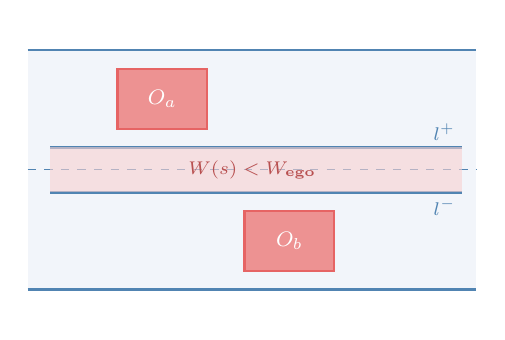
\begin{tikzpicture}[scale=0.95, transform shape]
  % 统一边界框：与子图 a/c 对齐
  \useasboundingbox (0,-1.9) rectangle (6.0,1.9);

  \fill[bglight] (0,-1.6) rectangle (6.0,1.6);
  \draw[deepblue, thick] (0,-1.6) -- (6.0,-1.6);
  \draw[deepblue, thick] (0, 1.6) -- (6.0, 1.6);
  \draw[deepblue, dashed, thin] (0,0) -- (6.0,0);

  \fill[obsstatic] (1.2,0.55) rectangle (2.4,1.35);
  \node[white, font=\footnotesize\bfseries] at (1.8,0.95) {$O_a$};

  \fill[obsstatic] (2.9,-1.35) rectangle (4.1,-0.55);
  \node[white, font=\footnotesize\bfseries] at (3.5,-0.95) {$O_b$};

  \draw[deepblue, very thick] (0.3,0.3) -- (5.8,0.3);
  \node[deepblue, font=\scriptsize, right] at (5.3,0.5) {$l^+$};

  \draw[deepblue, very thick] (0.3,-0.3) -- (5.8,-0.3);
  \node[deepblue, font=\scriptsize, right] at (5.3,-0.5) {$l^-$};

  \fill[dangerred!30, opacity=0.6] (0.3,-0.3) rectangle (5.8,0.3);
  \node[dangerred!80!black, font=\scriptsize\bfseries] at (3.0,0) {$W(s)<W_{\text{ego}}$};
\end{tikzpicture}
}
  \column{0.38\textwidth}
  \small
  \textbf{现象}
  \begin{itemize}\setlength\itemsep{3pt}
    \item 每个障碍物独立决定左绕/右绕
    \item 左侧$O_1$：右绕$\to$上界下压
    \item 右侧$O_2$：左绕$\to$下界上抬
    \item 上下边界交叉$\to$BLOCKED
  \end{itemize}
  \vspace{0.4em}
  \textbf{根因}\\
  贪心策略不考虑障碍物间的\\空间耦合关系，缺乏全局视角
\end{columns}
\end{frame}

% ============================================================
% [05] 问题三：动态障碍物排除
% ============================================================
\begin{frame}{Apollo问题三：动态障碍物被路径阶段排除}
\begin{columns}[T,onlytextwidth]
  \column{0.6\textwidth}
  \centering
  \adjustbox{max width=\linewidth, max totalheight=0.82\textheight}{% 问题三 动态障碍物排除（子图 c）
\begin{tikzpicture}[scale=0.95, transform shape]
  % 统一边界框：与子图 a/b 对齐
  \useasboundingbox (0,-1.9) rectangle (6.0,1.9);

  % 道路
  \fill[bglight] (0,-1.8) rectangle (6.0,1.8);
  \draw[deepblue, thick] (0,-1.8) -- (6.0,-1.8);
  \draw[deepblue, thick] (0, 1.8) -- (6.0, 1.8);
  \draw[deepblue, dashed, thin] (0,0) -- (6.0,0);

  % 行人（动态障碍物）
  \fill[obsdyn] (3.5,0.1) rectangle (4.0,0.7);
  \draw[-Stealth, thick, dangerred] (3.75,0.7) -- (3.75,1.4);
  \node[font=\scriptsize, dangerred!70!black, right] at (4.1,1.15) {行人 1.2m/s};

  % Path阶段排除标记：× 叠在行人上，文字移到道路内右上方
  \node[dangerred, font=\Large, opacity=0.85] at (3.75,0.4) {\textbf{$\times$}};
  \node[font=\scriptsize, dangerred!80!black, right] at (4.1,0.4) {Path阶段排除};

  % 自车
  \fill[deepblue] (0.6,-0.35) rectangle (1.2,0.35);
  \node[deepblue, font=\tiny, below] at (0.9,-0.4) {自车};
  \draw[-Stealth, thick, deepblue] (1.3,0) -- (3.2,0);
  \node[font=\scriptsize, deepblue, above] at (2.25,0.05) {8 m/s};

  % Speed阶段才发现标注
  \draw[dangerred, very thick, dashed] (3.2,-0.6) rectangle (4.3,0.9);
  \node[dangerred, font=\scriptsize\bfseries] at (2.2,-1.25) {Speed阶段才发现};
  \draw[dangerred, thin] (3.0,-1.15) -- (3.2,-0.7);

\end{tikzpicture}
}
  \column{0.38\textwidth}
  \small
  \textbf{现象}
  \begin{itemize}\setlength\itemsep{3pt}
    \item 路径阶段只处理静态障碍物
    \item 行人/自行车被过滤
    \item 路径直行$\to$速度阶段才发现
    \item 被迫急刹或停车
  \end{itemize}
  \vspace{0.4em}
  \textbf{根因}\\
  Path与Speed解耦架构中，\\动态目标信息无法从Speed\\反馈到Path，约束传递断裂
\end{columns}
\end{frame}

% ============================================================
% [06] MIKU 三项改进总览
% ============================================================
\begin{frame}{MIKU算法：三项改进总览}
\begin{columns}[T,onlytextwidth]
  \column{0.6\textwidth}
  \centering
  \adjustbox{max width=\linewidth, max totalheight=0.82\textheight}{% MIKU 多障碍物统一规划算法总流程
\begin{tikzpicture}[
    scale=1.0, transform shape,
    stepimp/.style={rectangle, rounded corners=3pt, draw=deeppink, fill=improvedpink, minimum width=5.4cm, minimum height=1.0cm, font=\small, align=center},
    inp/.style={rectangle, draw=deepblue, fill=inputyellow, minimum width=4.0cm, minimum height=0.8cm, font=\footnotesize, align=center},
    outnode/.style={rectangle, rounded corners=3pt, draw=deeppink, fill=outputpink, minimum width=4.0cm, minimum height=0.8cm, font=\small\bfseries, align=center},
    qpnode/.style={rectangle, rounded corners=3pt, draw=deepblue, fill=lightblue, minimum width=4.0cm, minimum height=0.8cm, font=\small\bfseries, align=center},
    arr/.style={-Stealth, thick, deepblue},
    injarr/.style={-Stealth, thick, deeppink},
]

% 输入
\node[inp] (i1) at (-5.8, 6.0) {参考线 $+$ 障碍物集合};
\node[inp] (i2) at (-5.8, 5.0) {预测轨迹 $+$ 车辆状态};

% 步骤（间距 1.7，全部为 MIKU 改进）
\node[stepimp] (s1) at (0, 5.5)  {\textbf{Step 1} 到达时间 $\tau(s)$ 与时变 SL 投影};
\node[stepimp] (s2) at (0, 3.8)  {\textbf{Step 2} 多因子威胁度评估 $\Theta_i$};
\node[stepimp] (s3) at (0, 2.1)  {\textbf{Step 3} 动态安全裕度 $\delta_i$ 与边界 $u_i,v_i$};
\node[stepimp] (s4) at (0, 0.4)  {\textbf{Step 4} 扫描线重叠分组 $\mathcal{G}_1,\ldots,\mathcal{G}_m$};
\node[stepimp] (s5) at (0,-1.3)  {\textbf{Step 5} 组内最大间隙 $g^\star_j=\max_k g_{j,k}$};
\node[stepimp] (s6) at (0,-3.0)  {\textbf{Step 6} 合并全局路径横向边界};
\node[stepimp] (s7) at (0,-4.7)  {\textbf{Step 7} ST 时空可通行走廊 $\Omega$};

% 输出（左侧）与跨接口的速度 QP
\node[outnode] (o1) at (-5.8,-3.0) {路径横向边界};
\node[outnode] (o2) at (-5.8,-4.7) {时空可通行走廊};
\node[qpnode]  (qp) at (-5.8,-6.4) {速度 QP（求解器不变）};

% 输入箭头
\draw[arr] (i1.east) -- (s1.west);
\draw[arr] (i2.east) -- (s1.west);

% 步骤间箭头
\draw[arr] (s1) -- (s2);
\draw[arr] (s2) -- (s3);
\draw[arr] (s3) -- (s4);
\draw[arr] (s4) -- (s5);
\draw[arr] (s5) -- (s6);
\draw[arr] (s6) -- (s7);

% 输出箭头
\draw[arr] (s6.west) -- (o1.east);
\draw[arr] (s7.west) -- (o2.east);

% 走廊注入速度 QP（跨解耦接口）
\draw[injarr] (o2.south) -- node[right, font=\footnotesize, deeppink] {逐时间步纵向上界} (qp.north);

\end{tikzpicture}
}
  \column{0.38\textwidth}
  \small
  \textbf{设计原则}
  \begin{itemize}\setlength\itemsep{3pt}
    \item 三项改进一一对应三类问题
    \item 共享统一数学符号$(u_i, v_i, \delta, \tau)$
    \item 仅改动PathBoundsDecider一步
    \item 下游QP/Control零改动
  \end{itemize}
  \vspace{0.4em}
  \textbf{MIKU = }\\
  \textbf{M}ulti-obstacle\\
  \textbf{I}nteraction-aware\\
  \textbf{K}inematic\\
  \textbf{U}nified planner
\end{columns}
\end{frame}

% ============================================================
% [07] 改进一：差异化安全距离
% ============================================================
\begin{frame}{改进一：多因子威胁度与差异化安全距离}
\begin{columns}[T,onlytextwidth]
  \column{0.48\textwidth}
  \centering
  \adjustbox{max width=\linewidth, max totalheight=0.6\textheight}{% 路锥场景：差异化 d_buf=0.15m，恰好可通行（子图 a）
\begin{tikzpicture}[scale=1.0, transform shape]
  \useasboundingbox (-0.3,-2.4) rectangle (8.1,2.4);
  % 隐形占位点：强制两个子图 pdfcrop 裁剪后宽度一致
  \draw[opacity=0] (-0.3,-2.4) rectangle (8.1,2.4);

  % 背景
  \fill[bglight] (0,-2.3) rectangle (7.0,2.3);

  % 道路边界 ±1.875m
  \draw[deepblue, very thick] (0,-1.875) -- (7.0,-1.875);
  \draw[deepblue, very thick] (0, 1.875) -- (7.0, 1.875);
  \draw[deepblue, dashed, thin] (0,0) -- (7.0,0);

  % 车道宽度标注
  \draw[{Stealth}-{Stealth}, thin, deepblue] (0.3,-1.875) -- (0.3,1.875);
  \node[font=\scriptsize, deepblue, rotate=90] at (0.6,0) {车道 3.75m};

  % 路锥（宽0.3m，高0.3m，中心在 (3.25, -0.225)）
  \fill[dangerred!70, draw=dangerred, thick] (3.1,-0.375) rectangle (3.4,-0.075);
  \node[white, font=\tiny\bfseries] at (3.25,-0.225) {锥};

  % 缓冲区 d_buf=0.15m
  \draw[dangerred!70, dashed, thick] (2.95,-0.525) rectangle (3.55,0.075);
  \node[dangerred!70!black, font=\scriptsize, anchor=west] at (3.7,-0.225)
    {$\delta{=}0.15$m};

  % 膨胀距离标注
  \draw[{Stealth}-{Stealth}, dangerred!60, thin] (2.8,-0.375) -- (2.8,-0.525);
  \node[dangerred!60, font=\tiny, left] at (2.75,-0.45) {0.15};
  \draw[{Stealth}-{Stealth}, dangerred!60, thin] (2.8,-0.075) -- (2.8,0.075);
  \node[dangerred!60, font=\tiny, left] at (2.75,0.0) {0.15};

  % 通行区域 [0.075, 1.875]
  \fill[lightgreen, opacity=0.25] (1.0,0.075) rectangle (5.5,1.875);

  % 自车
  \fill[deepblue, opacity=0.3] (1.0,0.075) rectangle (5.5,1.875);
  \draw[deepblue, thick, rounded corners=2pt] (1.0,0.075) rectangle (5.5,1.875);
  \node[deepblue, font=\scriptsize\bfseries] at (3.25,0.975) {自车};

  % 净间距标注
  \draw[{Stealth}-{Stealth}, thick, lightgreen!60!black] (6.2,0.075) -- (6.2,1.875);
  \node[font=\scriptsize, lightgreen!60!black, anchor=west] at (6.3,0.975) {1.80m};
  \node[font=\scriptsize, lightgreen!60!black, anchor=west] at (6.3,0.55) {$= W_{\mathrm{ego}}$};

  \node[lightgreen!60!black, font=\normalsize\bfseries] at (1.5,-2.1) {$\checkmark$};
\end{tikzpicture}
}\\[2pt]
  {\footnotesize (a) 差异化$\delta_i$：低威胁路锥缩小缓冲}
  \column{0.48\textwidth}
  \centering
  \adjustbox{max width=\linewidth, max totalheight=0.6\textheight}{% 路锥场景：Apollo d_buf=0.3m，BLOCKED（子图 b）
\begin{tikzpicture}[scale=1.0, transform shape]
  \useasboundingbox (-0.3,-2.4) rectangle (8.1,2.4);
  % 隐形占位点：强制两个子图 pdfcrop 裁剪后宽度一致
  \draw[opacity=0] (-0.3,-2.4) rectangle (8.1,2.4);

  % 背景
  \fill[bglight] (0,-2.3) rectangle (7.0,2.3);

  % 道路边界 ±1.875m
  \draw[deepblue, very thick] (0,-1.875) -- (7.0,-1.875);
  \draw[deepblue, very thick] (0, 1.875) -- (7.0, 1.875);
  \draw[deepblue, dashed, thin] (0,0) -- (7.0,0);

  % 车道宽度标注
  \draw[{Stealth}-{Stealth}, thin, deepblue] (0.3,-1.875) -- (0.3,1.875);
  \node[font=\scriptsize, deepblue, rotate=90] at (0.6,0) {车道 3.75m};

  % 路锥
  \fill[dangerred!70, draw=dangerred, thick] (3.1,-0.375) rectangle (3.4,-0.075);
  \node[white, font=\tiny\bfseries] at (3.25,-0.225) {锥};

  % 缓冲区 d_buf=0.3m
  \draw[dangerred!70, dashed, thick] (2.8,-0.675) rectangle (3.7,0.225);
  \node[dangerred!70!black, font=\scriptsize, anchor=west] at (3.85,-0.225)
    {$\delta{=}0.3$m};

  % 膨胀距离标注
  \draw[{Stealth}-{Stealth}, dangerred!60, thin] (2.6,-0.375) -- (2.6,-0.675);
  \node[dangerred!60, font=\tiny, left] at (2.55,-0.525) {0.3};
  \draw[{Stealth}-{Stealth}, dangerred!60, thin] (2.6,-0.075) -- (2.6,0.225);
  \node[dangerred!60, font=\tiny, left] at (2.55,0.075) {0.3};

  % 上方不足区域 1.65m
  \fill[dangerred, opacity=0.12] (1.0,0.225) rectangle (5.5,1.875);
  % 下方不足区域 1.2m
  \fill[dangerred, opacity=0.12] (1.0,-1.875) rectangle (5.5,-0.675);

  % 上方净间距
  \draw[{Stealth}-{Stealth}, thick, dangerred] (5.7,0.225) -- (5.7,1.875);
  \node[font=\scriptsize, dangerred, anchor=west] at (5.8,1.05) {1.65m};
  \node[font=\scriptsize, dangerred, anchor=west] at (5.8,0.65) {$< W_{\mathrm{ego}}$};

  % 下方净间距
  \draw[{Stealth}-{Stealth}, thick, dangerred] (5.7,-1.875) -- (5.7,-0.675);
  \node[font=\scriptsize, dangerred, anchor=west] at (5.8,-1.275) {1.20m};
  \node[font=\scriptsize, dangerred, anchor=west] at (5.8,-1.6) {$< W_{\mathrm{ego}}$};

  % BLOCKED
  \draw[dangerred, ultra thick] (2.5,1.0) -- (4.0,-1.0);
  \draw[dangerred, ultra thick] (2.5,-1.0) -- (4.0,1.0);
  \node[dangerred, font=\small\bfseries] at (3.25,-2.1) {BLOCKED};
\end{tikzpicture}
}\\[2pt]
  {\footnotesize (b) 统一$\delta$：通行带被压缩为零}
\end{columns}
\vspace{0.3em}
\small
\begin{itemize}\setlength\itemsep{2pt}
  \item 五因子融合：TTC、横向重叠率、相对速度、障碍物类型、交互密度$\to$威胁度$\Theta_i\in[0,1]$
  \item 输出：$\delta_i = \delta_{\min} + (\delta_{\max}-\delta_{\min})\cdot\Theta_i$，低威胁缩小缓冲释放通行空间
\end{itemize}
\end{frame}

% ============================================================
% [08] 改进二：组级最大间隙
% ============================================================
\begin{frame}{改进二：扫描线分组与最大间隙策略}
\begin{columns}[T,onlytextwidth]
  \column{0.55\textwidth}
  \centering
  \adjustbox{max width=\linewidth, max totalheight=0.78\textheight}{% 引理1+定理1 几何图证（1D 横向数轴）
\begin{tikzpicture}[scale=1.0, transform shape]

% 障碍物位置设计: g₂ 为最大间隙
% O₁@1.5, O₂@3.0, O₃@6.5, O₄@8.0 (中心)
% 半宽 0.35, δ 扩展 0.55
% l_road⁻=0, l_road⁺=9.5

% === 上图: 排序后的障碍物横向投影 ===

% 道路区域淡色背景（先画，避免盖住坐标轴）
\fill[bglight] (0,-0.7) rectangle (9.5,0.7);

% l 轴
\draw[->, thick] (-0.5,0) -- (10.2,0) node[right,font=\footnotesize] {$l$};

% 道路边界（垂直于 l 轴的竖线）
\draw[deepblue, very thick] (0,-0.9) -- (0,0.9);
\node[deepblue, font=\scriptsize, below] at (0,-0.95) {$l_{road}^-$};
\draw[deepblue, very thick] (9.5,-0.9) -- (9.5,0.9);
\node[deepblue, font=\scriptsize, below] at (9.5,-0.95) {$l_{road}^+$};

% 4 个障碍物（按 u_i 排序）
\fill[obsstatic] (1.15,-0.35) rectangle (1.85,0.35);
\node[white, font=\scriptsize\bfseries] at (1.5,0) {$O_1$};

\fill[obsstatic] (2.65,-0.35) rectangle (3.35,0.35);
\node[white, font=\scriptsize\bfseries] at (3.0,0) {$O_2$};

\fill[obsstatic] (6.15,-0.35) rectangle (6.85,0.35);
\node[white, font=\scriptsize\bfseries] at (6.5,0) {$O_3$};

\fill[obsstatic] (7.65,-0.35) rectangle (8.35,0.35);
\node[white, font=\scriptsize\bfseries] at (8.0,0) {$O_4$};

% u_i / v_i 膨胀区
\draw[obsbuf, dashed] (0.95,-0.55) rectangle (2.05,0.55);
\draw[obsbuf, dashed] (2.45,-0.55) rectangle (3.55,0.55);
\draw[obsbuf, dashed] (5.95,-0.55) rectangle (7.05,0.55);
\draw[obsbuf, dashed] (7.45,-0.55) rectangle (8.55,0.55);

% u_i / v_i 标注（选择性标注避免拥挤）
\node[deepblue, font=\tiny] at (0.95,0.75) {$u_1$};
\node[deeppink, font=\tiny] at (2.05,0.75) {$v_1$};
\node[deepblue, font=\tiny] at (2.45,0.75) {$u_2$};
\node[deeppink, font=\tiny] at (3.55,0.75) {$v_2$};
\node[deepblue, font=\tiny] at (5.95,0.75) {$u_3$};
\node[deeppink, font=\tiny] at (7.05,0.75) {$v_3$};
\node[deepblue, font=\tiny] at (7.45,0.75) {$u_4$};
\node[deeppink, font=\tiny] at (8.55,0.75) {$v_4$};

% 5 个间隙标注（在下方）
% g₀ = u₁ - l_road⁻ = 0.95
\draw[<->, thick, lightgreen!60!black] (0,-1.2) -- (0.95,-1.2);
\node[font=\scriptsize, lightgreen!60!black] at (0.475,-1.5) {$g_0$};

% g₁ = u₂ - v₁ = 0.40
\draw[<->, thick, lightgreen!60!black] (2.05,-1.2) -- (2.45,-1.2);
\node[font=\scriptsize, lightgreen!60!black] at (2.25,-1.5) {$g_1$};

% g₂ = u₃ - v₂ = 2.40 ← 最大间隙
\draw[<->, very thick, deeppink] (3.55,-1.2) -- (5.95,-1.2);
\node[font=\small\bfseries, deeppink] at (4.75,-1.5) {$g_2^\star$};

% g₃ = u₄ - v₃ = 0.40
\draw[<->, thick, lightgreen!60!black] (7.05,-1.2) -- (7.45,-1.2);
\node[font=\scriptsize, lightgreen!60!black] at (7.25,-1.5) {$g_3$};

% g₄ = l_road⁺ - v₄ = 0.95
\draw[<->, thick, lightgreen!60!black] (8.55,-1.2) -- (9.5,-1.2);
\node[font=\scriptsize, lightgreen!60!black] at (9.025,-1.5) {$g_4$};

% 最优分割线
\draw[deeppink, thick, dashed] (4.75,-0.9) -- (4.75,0.9);

\node[font=\scriptsize] at (4.75,-1.9) {$k{=}4$ 个障碍物，$k{+}1{=}5$ 个候选间隙，$g_2^\star$ 最大};

% === 下图: 决策向量 ===
\begin{scope}[shift={(0,-3.8)}]

  % R 群背景
  \fill[lightgreen!20] (0,-0.6) rectangle (4.75,0.6);
  % L 群背景
  \fill[improvedpink!25] (4.75,-0.6) rectangle (9.5,0.6);

  % 4 个障碍物
  \fill[obsstatic] (1.15,-0.35) rectangle (1.85,0.35);
  \node[white, font=\scriptsize\bfseries] at (1.5,0) {$O_1$};
  \node[deepblue, font=\scriptsize\bfseries] at (1.5,-0.65) {$d_1{=}R$};

  \fill[obsstatic] (2.65,-0.35) rectangle (3.35,0.35);
  \node[white, font=\scriptsize\bfseries] at (3.0,0) {$O_2$};
  \node[deepblue, font=\scriptsize\bfseries] at (3.0,-0.65) {$d_2{=}R$};

  \fill[obsstatic] (6.15,-0.35) rectangle (6.85,0.35);
  \node[white, font=\scriptsize\bfseries] at (6.5,0) {$O_3$};
  \node[deeppink, font=\scriptsize\bfseries] at (6.5,-0.65) {$d_3{=}L$};

  \fill[obsstatic] (7.65,-0.35) rectangle (8.35,0.35);
  \node[white, font=\scriptsize\bfseries] at (8.0,0) {$O_4$};
  \node[deeppink, font=\scriptsize\bfseries] at (8.0,-0.65) {$d_4{=}L$};

  % 分割线
  \draw[deeppink, thick, dashed] (4.75,-0.8) -- (4.75,0.8);
  \node[deeppink, font=\scriptsize] at (4.75,1.0) {$p^\star{=}2$};

  % 群标注
  \node[deepblue, font=\scriptsize] at (2.25,-1.1) {$\mathcal{R}{=}\{O_1,O_2\}$};
  \node[deeppink, font=\scriptsize] at (7.25,-1.1) {$\mathcal{L}{=}\{O_3,O_4\}$};

  % 连续性说明
  \node[font=\scriptsize] at (4.75,-1.5) {$\mathbf{d}^\star{=}(R,R,L,L)$，排序中连续，无交错};
\end{scope}

\end{tikzpicture}
}
  \column{0.43\textwidth}
  \small
  \begin{itemize}\setlength\itemsep{3pt}
    \item 扫描线检测纵向重叠$\to$连通分量分组
    \item 组内按$u_i$排序，枚举$k{+}1$个间隙
    \item 选最大间隙$g_{p^*}$穿过
    \item 搜索空间$2^k\to k{+}1$
    \item 复杂度$O(k\log k)$
  \end{itemize}
  \vspace{0.4em}
  \textbf{最优性保证}\\
  引理+定理证明$W(p)=g_p$\\
  选最大$g_p$即精确最优\\
  （详见下页证明）
\end{columns}
\end{frame}

% ============================================================
% [08b] 最优性证明（供老师阅读）
% ============================================================
\begin{frame}{最大间隙最优性证明}
\small
\textbf{引理}（最优分割连续性）\quad
按$u_i$升序排列后，存在最优解$\mathbf{d}^*$使分割连续：$\exists\, p$，使$d_{(i)}^*=L,\;\forall i\leq p$；$d_{(i)}^*=R,\;\forall i>p$。

\vspace{0.3em}
\textit{证明要点}：取任意最优解，令$\beta=\min_{i\in\mathcal{R}}u_i$，将所有$u_i\geq\beta$且原属$\mathcal{L}$的障碍物移入$\mathcal{R}$。$\min_{\mathcal{R}}u_i$不变，$\max_{\mathcal{L}}v_i$不增$\Rightarrow$通行带宽度不减，仍为最优。移动后分割在排序中连续。$\Box$

\vspace{0.5em}
\textbf{定理}（最大间隙最优性）\quad
定义前缀安全边界$V_p=\max_{q\leq p}v_{(q)}$，间隙
\[
g_p = \begin{cases}
  u_{(1)}-l_{road}^- & p=0\\
  u_{(p+1)}-V_p & 1\leq p\leq k{-}1\\
  l_{road}^+-V_k & p=k
\end{cases}
\]
则通行带宽度$W(p)=g_p$，最优宽度$W^*=\max_p g_p$。

\vspace{0.3em}
\textit{证明要点}：对$p=0,1,\ldots,k$逐一代入上下界表达式验证$W(p)=g_p$成立。选最大$g_p$即为最优。$\Box$
\end{frame}

% ============================================================
% [09] 改进三：时空走廊
% ============================================================
\begin{frame}{改进三：时空可通行走廊与路径-速度协调}
\begin{columns}[T,onlytextwidth]
  \column{0.48\textwidth}
  \centering
  \adjustbox{max width=\linewidth, max totalheight=0.6\textheight}{% 图6(a) 车道汇入·Baseline：汇入车 ST 轨迹为倾斜平行四边形，
% 全时刻并集投影把其左沿保守压至 t=0，自车从起点即被挡，被迫停车。
\begin{tikzpicture}[scale=1.0, transform shape, arr/.style={-Stealth, thick}]
  \useasboundingbox (-0.75,-1.05) rectangle (5.85,4.75);

  % 汇入车 ST 轨迹：倾斜平行四边形，左沿压至 t=0（左下角 (0,1.2)）
  \fill[dangerred!35, draw=dangerred, thick]
    (0,1.2) -- (4.0,3.3) -- (4.0,4.3) -- (0,2.2) -- cycle;
  \node[font=\scriptsize\bfseries, dangerred!85!black, rotate=27] at (2.0,3.0) {汇入车 ST 轨迹};
  % 压至 t=0 标注
  \draw[dangerred, very thick] (0,1.2) -- (0,2.2);
  \node[font=\tiny, dangerred!80!black, anchor=east, align=right] at (-0.05,1.7) {左沿\\压至\\$t{=}0$};

  % 坐标轴
  \draw[arr] (0,0) -- (5.6,0) node[right, font=\scriptsize] {$t$/s};
  \draw[arr] (0,0) -- (0,4.5) node[above, font=\scriptsize] {$s$/m};
  \node[font=\tiny, left=2pt] at (0,0) {$0$};

  % Baseline s(t)：起步即撞平行四边形下沿，被迫停车（几乎不前进）
  \draw[deepblue, very thick, -Stealth]
    (0,0) .. controls (0.3,0.6) and (0.6,0.95) .. (0.8,1.0) -- (5.0,1.0);
  \fill[deepblue] (0.8,1.0) circle (1.6pt);
  \node[font=\tiny, deepblue!80!black, anchor=north] at (2.8,0.97) {自车被迫停车（无通行区）};
\end{tikzpicture}
}\\[2pt]
  {\footnotesize (a) Baseline ST：独立障碍物边界}
  \column{0.48\textwidth}
  \centering
  \adjustbox{max width=\linewidth, max totalheight=0.6\textheight}{% 图6(b) 车道汇入·MIKU：按到达时间 τ(s) 摆放同一汇入车 ST 平行四边形，
% 其左沿右移至真实进入时刻，左下方让出三角通行区，自车得以争取一段前进。
\begin{tikzpicture}[scale=1.0, transform shape, arr/.style={-Stealth, thick}]
  \useasboundingbox (-0.75,-1.05) rectangle (5.85,4.75);

  % τ(s) 左下沿（楔形）：t≥τ(s) 可达
  \draw[deepblue, very thick, densely dashed] (0,0) -- (2.6,4.2);
  \node[font=\tiny, gray!55!black, align=center] at (0.55,3.75) {$t{<}\tau(s)$\\不可达};

  % 汇入车 ST 轨迹：同一平行四边形，左沿右移至 t=1.5（真实进入时刻）
  \fill[dangerred!35, draw=dangerred, thick]
    (1.5,1.2) -- (5.0,3.0) -- (5.0,4.0) -- (1.5,2.2) -- cycle;
  \node[font=\scriptsize\bfseries, dangerred!85!black, rotate=22] at (3.3,2.9) {汇入车 ST 轨迹};
  \draw[<-, dangerred!75!black, thin] (0.4,1.7) -- (1.45,1.7);
  \node[font=\tiny, dangerred!80!black, anchor=east, align=right] at (0.4,1.7) {左沿\\按 $\tau$\\右移};

  % 争取出的三角通行区（左下方）
  \fill[lightgreen!35] (0,0) -- (1.5,1.2) -- (1.5,0) -- cycle;
  \node[font=\tiny\bfseries, lightgreen!45!black, align=center] at (0.95,0.45) {通行区};

  % 坐标轴
  \draw[arr] (0,0) -- (5.6,0) node[right, font=\scriptsize] {$t$/s};
  \draw[arr] (0,0) -- (0,4.5) node[above, font=\scriptsize] {$s$/m};
  \node[font=\tiny, left=2pt] at (0,0) {$0$};

  % MIKU s(t)：沿通行区争取前进，随后与平行四边形下沿平行前进但保持间隙、不贴合
  \draw[deeppink, very thick, -Stealth]
    (0,0) .. controls (0.7,0.7) and (1.1,0.85) .. (1.4,0.9)
    .. controls (2.6,1.35) and (3.8,1.95) .. (5.0,2.45);
  \fill[deeppink] (1.4,0.9) circle (1.6pt);
  \node[font=\tiny, deeppink, anchor=north west] at (1.55,0.85) {争取前进后平行跟行};
  % 与下沿的间隙指示
  \draw[<->, gray!60, thin] (3.5,1.72) -- (3.5,2.28);
  \node[font=\tiny, gray!55!black, anchor=west] at (3.55,2.0) {间隙};
\end{tikzpicture}
}\\[2pt]
  {\footnotesize (b) MIKU ST：时空走廊约束注入}
\end{columns}
\vspace{0.3em}
\small
\begin{itemize}\setlength\itemsep{2pt}
  \item 到达时间函数$\tau(s)=\frac{-v_0+\sqrt{v_0^2+2as}}{a}$，查询行人在$t{=}\tau(s)$时的预测位置
  \item 走廊约束以ST上界注入速度QP，补上Path$\to$Speed缺失的约束传递通道
\end{itemize}
\end{frame}

% ============================================================
% [10] 实验一：差异化安全距离验证
% ============================================================
\begin{frame}{实验一：窄路双侧锥——差异化裕度验证}
\vspace{-0.4em}

\begin{center}
  \resizebox{0.50\paperwidth}{!}{\input{../图片/fig_exp_03_narrow_cones_sl_a}}\\[-3pt]
  {\footnotesize (a) Baseline：统一裕度$\to$BLOCKED}\\[1pt]
  \resizebox{0.50\paperwidth}{!}{\input{../图片/fig_exp_03_narrow_cones_sl_b}}\\[-3pt]
  {\footnotesize (b) MIKU：差异化裕度$\to$通行}
\end{center}

\begin{textblock*}{0.30\paperwidth}(0.68\paperwidth,0.64\paperheight)
  \begin{tcolorbox}[slideMetricCard,title=关键指标]
    \scriptsize\raggedright
    \textbf{结论：}差异化裕度释放窄路空间。\\
    P3：双侧各3锥，宽度临界\\
    Baseline：停车，$s_{end}$=\MThreeBaselineSEnd\,m\\
    MIKU：通过，$s_{end}$=\MThreeMikuSEnd\,m，$\bar{v}$=\MThreeMikuAvgV\,m/s\\
    QP：\MThreeBaselineQpTotal\,ms$\to$\MThreeMikuQpTotal\,ms
  \end{tcolorbox}
\end{textblock*}
\end{frame}

% ============================================================
% [11] 实验二：组级最大间隙验证
% ============================================================
\begin{frame}{实验二：施工区导流——最大间隙验证}
\vspace{-0.4em}

\begin{center}
  \resizebox{0.38\paperwidth}{!}{% 自动生成：请勿手动编辑。来源：图片/_gen_exp_figs.py
% 场景04 SL — 子图 a：Baseline
\def\datapath{data/04_dense_construction/}
\pgfplotsset{
    discard if not/.style 2 args={x filter/.code={
        \edef\tempa{\thisrow{#1}}\edef\tempb{#2}
        \ifx\tempa\tempb\else\def\pgfmathresult{nan}\fi
    }},
    discard if not2/.style n args={4}{x filter/.code={
        \edef\tempa{\thisrow{#1}}\edef\tempb{#2}
        \edef\tempc{\thisrow{#3}}\edef\tempd{#4}
        \ifx\tempa\tempb
            \ifx\tempc\tempd\else\def\pgfmathresult{nan}\fi
        \else\def\pgfmathresult{nan}\fi
    }}
}
\begin{tikzpicture}
\begin{axis}[
    width=0.9\linewidth, height=6.6cm,
    xlabel={$s$ (m)}, ylabel={$l$ (m)},
    xmin=0, xmax=85.0, ymin=-3.9, ymax=3.9,
    grid=both, grid style={gray!25},
    axis line style={thick},
    tick label style={font=\scriptsize},
    label style={font=\footnotesize},
    legend style={at={(0.98,0.02)}, anchor=south east, font=\scriptsize, draw=none, fill=white, fill opacity=0.85},
]
\addplot[fill=bglight, draw=none, forget plot, on layer=axis background] coordinates {(0,-1.875) (85.0,-1.875) (85.0,1.875) (0,1.875)} \closedcycle;
\addplot[fill=vibrantorange!25, draw=none, forget plot, on layer=axis background] coordinates {(0,1.875) (85.0,1.875) (85.0,3.750) (0,3.750)} \closedcycle;
\draw[black!55, semithick] (axis cs:0,-1.875) -- (axis cs:85.0,-1.875);
\draw[black!55, semithick] (axis cs:0,1.875) -- (axis cs:85.0,1.875);
\draw[black!30, dashed, thin] (axis cs:0,0) -- (axis cs:85.0,0);
% 可行带阴影（blocked 时按 blocked_s 截断）
\addplot[name path=lmin_baseline, draw=vibrantorange, thin, dashed, forget plot, unbounded coords=jump, restrict x to domain=0:23.000, ]
    table[col sep=comma, x=s, y=l_min, discard if not={mode}{baseline}] {\datapath sl.csv};
\addplot[name path=lmax_baseline, draw=vibrantorange, thin, dashed, forget plot, unbounded coords=jump, restrict x to domain=0:23.000, ]
    table[col sep=comma, x=s, y=l_max, discard if not={mode}{baseline}] {\datapath sl.csv};
\addplot[fill=lightgreen!35, draw=none, forget plot] fill between[of=lmin_baseline and lmax_baseline];
% 路径（blocked 时按 blocked_s 截断）
\addplot[deepblue, line width=2pt, unbounded coords=jump, restrict x to domain=0:23.000] table[col sep=comma, x=s, y=l_path, discard if not={mode}{baseline}] {\datapath sl.csv};
\addlegendentry{Baseline}
\addlegendimage{dangerred, thick, dashed}\addlegendentry{Trim @ $s$=23.0\,m}
\draw[dangerred, thick, dashed] (axis cs:23.000,-3.9) -- (axis cs:23.000,3.9);
\node[dangerred, font=\Large\bfseries, inner sep=0pt] at (axis cs:23.000,3.336) {$\times$};
% 障碍物 锥E1
\fill[dangerred!70, draw=dangerred, thick] (axis cs:14.750,-1.700) rectangle (axis cs:17.250,-1.300);
\node[anchor=south, font=\tiny, color=dangerred!80!black] at (axis cs:16.000,-1.000) {锥E1};
% 障碍物 锥E2
\fill[dangerred!70, draw=dangerred, thick] (axis cs:17.250,-1.050) rectangle (axis cs:19.750,-0.650);
\node[anchor=south, font=\tiny, color=dangerred!80!black] at (axis cs:18.500,-0.350) {锥E2};
% 障碍物 锥E3
\fill[dangerred!70, draw=dangerred, thick] (axis cs:19.750,-0.400) rectangle (axis cs:22.250,0.000);
\node[anchor=south, font=\tiny, color=dangerred!80!black] at (axis cs:21.000,0.300) {锥E3};
% 障碍物 锥E4
\fill[dangerred!70, draw=dangerred, thick] (axis cs:22.250,0.300) rectangle (axis cs:24.750,0.700);
\node[anchor=south, font=\tiny, color=dangerred!80!black] at (axis cs:23.500,1.000) {锥E4};
% 障碍物 锥E5
\fill[dangerred!70, draw=dangerred, thick] (axis cs:24.750,1.000) rectangle (axis cs:27.250,1.400);
\node[anchor=south, font=\tiny, color=dangerred!80!black] at (axis cs:26.000,1.700) {锥E5};
% 障碍物 水马M1
\fill[dangerred!70, draw=dangerred, thick] (axis cs:27.000,1.500) rectangle (axis cs:31.000,2.500);
\node[anchor=south, font=\tiny, color=dangerred!80!black] at (axis cs:29.000,2.800) {水马M1};
% 障碍物 水马M2
\fill[dangerred!70, draw=dangerred, thick] (axis cs:31.000,1.500) rectangle (axis cs:35.000,2.500);
\node[anchor=south, font=\tiny, color=dangerred!80!black] at (axis cs:33.000,2.800) {水马M2};
% 障碍物 水马M3
\fill[dangerred!70, draw=dangerred, thick] (axis cs:35.000,1.500) rectangle (axis cs:39.000,2.500);
\node[anchor=south, font=\tiny, color=dangerred!80!black] at (axis cs:37.000,2.800) {水马M3};
% 障碍物 水马M4
\fill[dangerred!70, draw=dangerred, thick] (axis cs:39.000,1.500) rectangle (axis cs:43.000,2.500);
\node[anchor=south, font=\tiny, color=dangerred!80!black] at (axis cs:41.000,2.800) {水马M4};
% 障碍物 水马M5
\fill[dangerred!70, draw=dangerred, thick] (axis cs:43.000,1.500) rectangle (axis cs:47.000,2.500);
\node[anchor=south, font=\tiny, color=dangerred!80!black] at (axis cs:45.000,2.800) {水马M5};
% 障碍物 水马M6
\fill[dangerred!70, draw=dangerred, thick] (axis cs:47.000,1.500) rectangle (axis cs:51.000,2.500);
\node[anchor=south, font=\tiny, color=dangerred!80!black] at (axis cs:49.000,2.800) {水马M6};
% 障碍物 水马M7
\fill[dangerred!70, draw=dangerred, thick] (axis cs:51.000,1.500) rectangle (axis cs:55.000,2.500);
\node[anchor=south, font=\tiny, color=dangerred!80!black] at (axis cs:53.000,2.800) {水马M7};
% 障碍物 水马M8
\fill[dangerred!70, draw=dangerred, thick] (axis cs:55.000,1.500) rectangle (axis cs:59.000,2.500);
\node[anchor=south, font=\tiny, color=dangerred!80!black] at (axis cs:57.000,2.800) {水马M8};
% 障碍物 锥X1
\fill[dangerred!70, draw=dangerred, thick] (axis cs:58.750,1.000) rectangle (axis cs:61.250,1.400);
\node[anchor=south, font=\tiny, color=dangerred!80!black] at (axis cs:60.000,1.700) {锥X1};
% 障碍物 锥X2
\fill[dangerred!70, draw=dangerred, thick] (axis cs:61.250,0.300) rectangle (axis cs:63.750,0.700);
\node[anchor=south, font=\tiny, color=dangerred!80!black] at (axis cs:62.500,1.000) {锥X2};
% 障碍物 锥X3
\fill[dangerred!70, draw=dangerred, thick] (axis cs:63.750,-0.400) rectangle (axis cs:66.250,0.000);
\node[anchor=south, font=\tiny, color=dangerred!80!black] at (axis cs:65.000,0.300) {锥X3};
% 障碍物 锥X4
\fill[dangerred!70, draw=dangerred, thick] (axis cs:66.250,-1.050) rectangle (axis cs:68.750,-0.650);
\node[anchor=south, font=\tiny, color=dangerred!80!black] at (axis cs:67.500,-0.350) {锥X4};
% 障碍物 锥X5
\fill[dangerred!70, draw=dangerred, thick] (axis cs:68.750,-1.700) rectangle (axis cs:71.250,-1.300);
\node[anchor=south, font=\tiny, color=dangerred!80!black] at (axis cs:70.000,-1.000) {锥X5};
\node[rectangle, fill=deepblue!75, draw=deepblue, thick, minimum width=18pt, minimum height=8pt, inner sep=0pt] (egobox) at (axis cs:0.000,0.000) {};
\fill[white] ([xshift=0pt]egobox.east) -- ([xshift=-3pt,yshift=2.5pt]egobox.east) -- ([xshift=-3pt,yshift=-2.5pt]egobox.east) -- cycle;
\node[anchor=south west, font=\tiny\bfseries, color=deepblue] at (axis cs:0.20,1.10) {EGO};
\end{axis}
\end{tikzpicture}
}\\[-3pt]
  {\footnotesize (a) Baseline：贪心冲突$\to$BLOCKED}\\[1pt]
  \resizebox{0.38\paperwidth}{!}{\input{../图片/fig_exp_04_dense_construction_sl_b}}\\[-3pt]
  {\footnotesize (b) MIKU：组级统一方向$\to$通行}
\end{center}

\begin{textblock*}{0.30\paperwidth}(0.68\paperwidth,0.64\paperheight)
  \begin{tcolorbox}[slideMetricCard,title=关键指标]
    \scriptsize\raggedright
    \textbf{结论：}组级方向统一，施工区保持通行。\\
    P4：18障碍物交错导流\\
    Baseline：停车，$s_{end}$=\MFourBaselineSEnd\,m\\
    MIKU：通过，$s_{end}$=\MFourMikuSEnd\,m，$\bar{v}$=\MFourMikuAvgV\,m/s\\
    QP：\MFourBaselineQpTotal\,ms$\to$\MFourMikuQpTotal\,ms
  \end{tcolorbox}
\end{textblock*}

\end{frame}

% ============================================================
% [12] 实验三：时空走廊验证
% ============================================================
\begin{frame}{实验三：行人横穿——时空走廊验证}
\vspace{-0.4em}

\begin{center}
  \resizebox{0.50\paperwidth}{!}{% 自动生成：请勿手动编辑。来源：图片/_gen_exp_figs.py
% 场景01 SL — 子图 a：Baseline
\def\datapath{data/01_crossing_ped/}
\pgfplotsset{
    discard if not/.style 2 args={x filter/.code={
        \edef\tempa{\thisrow{#1}}\edef\tempb{#2}
        \ifx\tempa\tempb\else\def\pgfmathresult{nan}\fi
    }},
    discard if not2/.style n args={4}{x filter/.code={
        \edef\tempa{\thisrow{#1}}\edef\tempb{#2}
        \edef\tempc{\thisrow{#3}}\edef\tempd{#4}
        \ifx\tempa\tempb
            \ifx\tempc\tempd\else\def\pgfmathresult{nan}\fi
        \else\def\pgfmathresult{nan}\fi
    }}
}
\begin{tikzpicture}
\begin{axis}[
    width=0.9\linewidth, height=4.2cm,
    xlabel={$s$ (m)}, ylabel={$l$ (m)},
    xmin=0, xmax=25.0, ymin=-2.2, ymax=2.2,
    grid=both, grid style={gray!25},
    axis line style={thick},
    tick label style={font=\scriptsize},
    label style={font=\footnotesize},
    legend style={at={(0.98,0.02)}, anchor=south east, font=\scriptsize, draw=none, fill=white, fill opacity=0.85},
]
\addplot[fill=bglight, draw=none, forget plot, on layer=axis background] coordinates {(0,-1.875) (25.0,-1.875) (25.0,1.875) (0,1.875)} \closedcycle;

\draw[black!55, semithick] (axis cs:0,-1.875) -- (axis cs:25.0,-1.875);
\draw[black!55, semithick] (axis cs:0,1.875) -- (axis cs:25.0,1.875);
\draw[black!30, dashed, thin] (axis cs:0,0) -- (axis cs:25.0,0);
% 可行带阴影（blocked 时按 blocked_s 截断）
\addplot[name path=lmin_baseline, draw=vibrantorange, thin, dashed, forget plot, ]
    table[col sep=comma, x=s, y=l_min, discard if not={mode}{baseline}] {\datapath sl.csv};
\addplot[name path=lmax_baseline, draw=vibrantorange, thin, dashed, forget plot, ]
    table[col sep=comma, x=s, y=l_max, discard if not={mode}{baseline}] {\datapath sl.csv};
\addplot[fill=lightgreen!35, draw=none, forget plot] fill between[of=lmin_baseline and lmax_baseline];
% 路径（blocked 时按 blocked_s 截断）
\addplot[deepblue, line width=2pt, unbounded coords=discard] table[col sep=comma, x=s, y=l_path, discard if not={mode}{baseline}] {\datapath sl.csv};
\addlegendentry{Baseline}


% 障碍物 行人
\fill[dangerred, opacity=0.95] (axis cs:12.000,-0.600) circle [radius=5pt];
\fill[dangerred, opacity=0.55] (axis cs:12.000,0.225) circle [radius=5pt];
\fill[dangerred, opacity=0.35] (axis cs:12.000,1.050) circle [radius=5pt];
\fill[dangerred, opacity=0.20] (axis cs:12.000,1.900) circle [radius=5pt];
\draw[->, dangerred, very thick, opacity=0.85] (axis cs:12.000,-0.600) -- (axis cs:12.000,1.900);
\node[anchor=south, font=\tiny, color=dangerred] at (axis cs:12.000,0.150) {行人 $v=(+0.0,+1.2)$};
\node[rectangle, fill=deepblue!75, draw=deepblue, thick, minimum width=18pt, minimum height=8pt, inner sep=0pt] (egobox) at (axis cs:0.000,0.000) {};
\fill[white] ([xshift=0pt]egobox.east) -- ([xshift=-3pt,yshift=2.5pt]egobox.east) -- ([xshift=-3pt,yshift=-2.5pt]egobox.east) -- cycle;
\node[anchor=south west, font=\tiny\bfseries, color=deepblue] at (axis cs:0.20,1.10) {EGO};
\end{axis}
\end{tikzpicture}
}\\[-3pt]
  {\footnotesize (a) Baseline：路径阶段行人不可见}\\[1pt]
  \resizebox{0.50\paperwidth}{!}{% 自动生成：请勿手动编辑。来源：图片/_gen_exp_figs.py
% 场景01 SL — 子图 b：MIKU
\def\datapath{data/01_crossing_ped/}
\pgfplotsset{
    discard if not/.style 2 args={x filter/.code={
        \edef\tempa{\thisrow{#1}}\edef\tempb{#2}
        \ifx\tempa\tempb\else\def\pgfmathresult{nan}\fi
    }},
    discard if not2/.style n args={4}{x filter/.code={
        \edef\tempa{\thisrow{#1}}\edef\tempb{#2}
        \edef\tempc{\thisrow{#3}}\edef\tempd{#4}
        \ifx\tempa\tempb
            \ifx\tempc\tempd\else\def\pgfmathresult{nan}\fi
        \else\def\pgfmathresult{nan}\fi
    }}
}
\begin{tikzpicture}
\begin{axis}[
    width=0.9\linewidth, height=4.2cm,
    xlabel={$s$ (m)}, ylabel={$l$ (m)},
    xmin=0, xmax=25.0, ymin=-2.2, ymax=2.2,
    grid=both, grid style={gray!25},
    axis line style={thick},
    tick label style={font=\scriptsize},
    label style={font=\footnotesize},
    legend style={at={(0.98,0.02)}, anchor=south east, font=\scriptsize, draw=none, fill=white, fill opacity=0.85},
]
\addplot[fill=bglight, draw=none, forget plot, on layer=axis background] coordinates {(0,-1.875) (25.0,-1.875) (25.0,1.875) (0,1.875)} \closedcycle;

\draw[black!55, semithick] (axis cs:0,-1.875) -- (axis cs:25.0,-1.875);
\draw[black!55, semithick] (axis cs:0,1.875) -- (axis cs:25.0,1.875);
\draw[black!30, dashed, thin] (axis cs:0,0) -- (axis cs:25.0,0);
% 可行带阴影（blocked 时按 blocked_s 截断）
\addplot[name path=lmin_miku, draw=vibrantorange, thin, dashed, forget plot, ]
    table[col sep=comma, x=s, y=l_min, discard if not={mode}{miku}] {\datapath sl.csv};
\addplot[name path=lmax_miku, draw=vibrantorange, thin, dashed, forget plot, ]
    table[col sep=comma, x=s, y=l_max, discard if not={mode}{miku}] {\datapath sl.csv};
\addplot[fill=lightgreen!35, draw=none, forget plot] fill between[of=lmin_miku and lmax_miku];
% 路径（blocked 时按 blocked_s 截断）
\addplot[vibrantgreen, line width=2pt, unbounded coords=discard] table[col sep=comma, x=s, y=l_path, discard if not={mode}{miku}] {\datapath sl.csv};
\addlegendentry{MIKU}


% 障碍物 行人：t=0 起点淡出扫掠 + τ(12) 到达时刻高亮位置
\fill[dangerred, opacity=0.30] (axis cs:12.000,-0.600) circle [radius=4pt];
\fill[dangerred, opacity=0.22] (axis cs:12.000,0.225) circle [radius=4pt];
\fill[dangerred, opacity=0.18] (axis cs:12.000,1.050) circle [radius=4pt];
\draw[->, dangerred, thick, opacity=0.55] (axis cs:12.000,-0.600) -- (axis cs:12.000,1.700);
\node[anchor=west, font=\tiny, color=dangerred, opacity=0.7] at (axis cs:12.15,-0.600) {$t{=}0$};
% τ(12)=1.5s 自车到达时刻行人实际位置 l=+1.275（上侧）
\fill[dangerred, opacity=0.95] (axis cs:12.000,1.275) circle [radius=5pt];
\draw[dangerred, thick] (axis cs:12.000,1.275) circle [radius=6.5pt];
\node[anchor=south west, font=\tiny\bfseries, color=dangerred] at (axis cs:12.15,1.275) {行人@$\tau{=}1.5$s};
% 自车贴下侧窄缝通过
\node[anchor=north, font=\tiny, color=vibrantgreen!60!black] at (axis cs:12.000,-0.72) {自车贴下侧过};
\node[rectangle, fill=deepblue!75, draw=deepblue, thick, minimum width=18pt, minimum height=8pt, inner sep=0pt] (egobox) at (axis cs:0.000,0.000) {};
\fill[white] ([xshift=0pt]egobox.east) -- ([xshift=-3pt,yshift=2.5pt]egobox.east) -- ([xshift=-3pt,yshift=-2.5pt]egobox.east) -- cycle;
\node[anchor=south west, font=\tiny\bfseries, color=deepblue] at (axis cs:0.20,1.10) {EGO};
\end{axis}
\end{tikzpicture}
}\\[-3pt]
  {\footnotesize (b) MIKU：$\tau(s)$投影后右偏绕行}
\end{center}

\begin{textblock*}{0.30\paperwidth}(0.68\paperwidth,0.64\paperheight)
  \begin{tcolorbox}[slideMetricCard,title=关键指标]
    \scriptsize\raggedright
    \textbf{结论：}行人入边界，提前绕行。\\
    P1：行人1.2\,m/s横穿\\
    Baseline：未到终点，$s_{end}$=\MOneBaselineSEnd\,m\\
    MIKU：通过，$s_{end}$=\MOneMikuSEnd\,m，$\bar{v}$=\MOneMikuAvgV\,m/s\\
    $|a_x|_{max}$：\MOneBaselineMaxAbsA$\to$\MOneMikuMaxAbsA\,m/s$^2$
  \end{tcolorbox}
\end{textblock*}
\end{frame}

% ============================================================
% [13] 消融实验
% ============================================================
\begin{frame}{消融实验：各组件必要性验证}
\adjustbox{max width=\linewidth, max totalheight=0.55\textheight}{\input{../图片/data/ablation/score_heatmap}}
\vspace{0.3em}
\small
\begin{itemize}\setlength\itemsep{2pt}
  \item 在4个压力场景上逐一关闭各组件（Leave-One-Out）
  \item 关闭时变投影/分组决策/差异化裕度中任一项$\to$至少1个场景失败
  \item 结论：三项路径组件互为必要条件，缺一不可
\end{itemize}
\end{frame}

% ============================================================
% [14] Dreamview在环演示
% ============================================================
\begin{frame}{Dreamview在环演示：C++接入后的规划行为}
\centering
\small

\centering\textbf{动态超车}\\[3pt]
\adjustbox{max width=0.5\linewidth}{\input{../图片/fig_eng_scn01_dreamview_b}}\\[2pt]
{\footnotesize 借道超越慢车}


\centering\textbf{窄路通行}\\[3pt]
\adjustbox{max width=0.5\linewidth}{\input{../图片/fig_eng_scn02_dreamview_b}}\\[2pt]
{\footnotesize 差异化裕度穿越锥列}


\centering\textbf{单车道封闭导流}\\[3pt]
\adjustbox{max width=0.5\linewidth}{\input{../图片/fig_eng_scn03_dreamview_b}}\\[2pt]
{\footnotesize 组级决策统一左绕}

{\footnotesize 三个场景均在Apollo 11.0 C++工程中运行，MIKU路径边界分支通过配置开关启用，下游Control模块零改动。}
\end{frame}

% ============================================================
% [15] 总结与展望
% ============================================================
\begin{frame}{总结与展望}
\centering
\adjustbox{max width=\linewidth, max totalheight=0.88\textheight}{% 四项创新贡献汇总 四层堆叠结构
\begin{tikzpicture}[scale=0.9, transform shape,
    layer/.style={rectangle, rounded corners=4pt, draw=deeppink, fill=improvedpink, minimum width=8cm, minimum height=1.2cm, font=\small\bfseries, align=center},
    capbadge/.style={rectangle, rounded corners=3pt, draw=deeppink, fill=deeppink, text=white, minimum width=2.0cm, minimum height=0.7cm, font=\small\bfseries, align=center},
]

\node[layer] (sys)    at (0,6) {ST 走廊与速度规划协调};
\node[capbadge]       at (-5.5,6) {系统};

\node[layer] (safety) at (0,4) {威胁度分级与动态安全距离};
\node[capbadge]       at (-5.5,4) {安全};

\node[layer] (algo)   at (0,2) {扫描线分组与时变 SL 投影};
\node[capbadge]       at (-5.5,2) {算法};

\node[layer] (theory) at (0,0) {最大间隙最优性定理};
\node[capbadge]       at (-5.5,0) {理论};

\draw[-Stealth, very thick, deeppink] (theory.north) -- (algo.south);
\draw[-Stealth, very thick, deeppink] (algo.north)   -- (safety.south);
\draw[-Stealth, very thick, deeppink] (safety.north) -- (sys.south);

\end{tikzpicture}
}
\end{frame}


% ============================================================
% [16] 结束
% ============================================================
\begin{frame}
  \vfill
  \vspace*{0.35cm}
  \begin{center}
    {\Huge 恳请各位老师批评指正}
  \end{center}
  \vfill
\end{frame}

\end{document}
